\documentclass[journal]{vgtc}                % final (journal style)

%% These few lines make a distinction between latex and pdflatex calls and they
%% bring in essential packages for graphics and font handling.
%% Note that due to the \DeclareGraphicsExtensions{} call it is no longer necessary
%% to provide the the path and extension of a graphics file:
%% 
\includegraphics{diamondrule} is completely sufficient.
%%
\ifpdf%                                % if we use pdflatex
  \pdfoutput=1\relax                   % create PDFs from pdfLaTeX
  \pdfcompresslevel=9                  % PDF Compression
  \pdfoptionpdfminorversion=7          % create PDF 1.7
  \ExecuteOptions{pdftex}
  \usepackage{graphicx}                % allow us to embed graphics files
  \DeclareGraphicsExtensions{.pdf,.png,.jpg,.jpeg} % for pdflatex we expect .pdf, .png, or .jpg files
\else%                                 % else we use pure latex
  \ExecuteOptions{dvips}
  \usepackage{graphicx}                % allow us to embed graphics files
  \DeclareGraphicsExtensions{.eps}     % for pure latex we expect eps files
\fi%

%% it is recomended to use ``\autoref{sec:bla}'' instead of ``Fig.~\ref{sec:bla}''
\graphicspath{ {pictures/} } % where to search for the images

\usepackage{microtype}                 % use micro-typography (slightly more compact, better to read)
\usepackage{hyperref}
\usepackage{listings}
\usepackage{cite}

\usepackage{tikz}
\usetikzlibrary{shapes.geometric, arrows}
\tikzstyle{startstop} = [rectangle, rounded corners, minimum width=3cm, minimum height=1cm,text centered, draw=black, fill=red!30]
\tikzstyle{io} = [trapezium, trapezium left angle=70, trapezium right angle=110, minimum width=3cm, minimum height=1cm, text centered, draw=black, fill=blue!30]\tikzstyle{process} = [rectangle, minimum width=3cm, minimum height=1cm, text centered, draw=black, fill=orange!30]
\tikzstyle{decision} = [diamond, minimum width=3cm, minimum height=1cm, text centered, draw=black, fill=green!30]
\tikzstyle{arrow} = [thick,->,>=stealth]


\PassOptionsToPackage{warn}{textcomp}  % to address font issues with \textrightarrow
\usepackage{times}                     % we use Times as the main font
\renewcommand*\ttdefault{txtt}         % a nicer typewriter font

%% declare the category of your paper, only shown in review mode
\vgtccategory{Research}

\title{How NBA Player Salaries Relate to Individual and Team Performance: Using Visualizations to Maximize a Team's Success}

\author{Alex Hoffer, Austin Nguyen, Prathveer Rai}

\abstract{
This paper attempts to describe how an NBA player's salary can be beneficial or detrimental to their team based on their performance in several statistical categories. This serves as a useful starting point for front office professionals employed by NBA teams who wish to make reasoned judgments about whether they should extend a player's contract or let them walk into free agency. After all, statistics in NBA basketball have become nuanced and sophisticated in the past decade, and teams such as the San Antonio Spurs have embraced their use and excel as a result. We believe that visualizations are the best method for truly understanding the effectiveness of an NBA player in the context of their salary since when these statistics are merely presented in their numerical form, people who are not mathematical experts (such as NBA General Managers, who are responsible for offering contracts to players) may not grasp the conclusion, or even worse, they may get the wrong impression about a certain player. Specifically, we believe that the radar chart is the most appropriate type of visualization to achieve this effect, since there are multiple statistical categories being judged by their relation to salary, which means it is essential that the user is able to see how far out edges extend within each category so they can conveniently visually compare how far out the edge pertaining to the salary is in relation to these statistics, giving them an indication of whether the player is worth their price.}




\date{\today}

\renewcommand{\manuscriptnotetxt}{}

\vgtcinsertpkg

\begin{document}

\maketitle

\section{Introduction}
Basketball players employed by the National Basketball Association (NBA) make a tremendous amount of money. Their agents negotiate with the general managers of professional teams in order to get a salary that they think their performance warrants. Unlike professional sports leagues like Major League Baseball (MLB), though, NBA teams have a \emph{salary cap}, which is a limit to the amount of money they can spend to field a 15-man teamof \$102 million. This means that it is within each NBA team's interests to pay each player in, the average case, the exact salary which fairly corresponds to their on-court performance and, in the best case scenario for the team, a salary that is as low as possible for a player that is extremely good. A good example of the latter case being beneficial to a team is Stephen Curry of the Golden State Warriors, who gets paid x/year, and yet is a two-time MVP who is commonly considered one of the best players of all time. This low salary allowed the Warriors to spend money on acquiring Kevin Durant, another MVP, for a max salary. 
\par Thus, this paper describes the process of our visualizations of the radar chart variety of specific players we believe are beneficial to observe in this way, since it has the capacity to captivate general managers of NBA teams into making the most reasoned decisions about who to sign and who to let walk in free agency. The paper will consist of several sections to achieve this effect, including the related visualizations we have found, the method we used to generate our visual computations, our programming implementation of these concepts, our results and their impact, and what we can conclude from our project and what future visualizations in this realm should address. 

\section{Related Work}
The use of spider charts to visualize NBA statistics is somewhat prevalent in the realm of entertainment, but not in information visualization research. 
\subsection{In Information Visualization Research}
Historically, academic publications in information visualization rarely tackle the topic of sports, much less spider charts devoted to NBA player statistics and their salary. However, over the past several years, this trend has begun to reverse, with conferences such as the IEEE VIS sponsoring workshops on sports data visualization, though the majority of these visualizations regard sports such as football, soccer, and baseball. Nevertheless, it is important for our purposes to survey the few visualizations within this subcategory of information visualization pertaining to the NBA that are present in academic research. \cite{chu}, a paper that introduces an interactive shot chart tool that allows the user to choose a player and see on a virtual basketball court the physical areas on the court where they perform best, presents the idea of using visualization to enhance our assessments of NBA players' in-game performances, but does not describe how tools like this could be used by NBA executives to make reasoned decisions about players' salaries. \cite{chen} proposes a new way of presenting post-game information, gravitating away from webcasts and towards "season level, game level, and session level" visualizations, but the purpose of this work is to augment the NBA fan's experience and, while this work does include some visualizations of performances that are relevant to our research, the purpose of such visualizations is for entertainment consumption and not for the maximization of team success. \cite{pagno} includes some visualizations that are similar to the ones we present in this work, including spider charts with steals, points, rebounds, assists, blocks, and turnovers as graph points of players such as Steve Nash, Deron Williams, and Rajon Rondo. However, these visualizations do not include player salary, which means they do not explore the financial implications of player performance that come in handy when making player personnel decisions. \cite{reyna} uses line graphs and bar graphs to visualize and compare team performances, but provides no application of the importance of such visualizations to executive decision making nor does it provide visualizations of individual player performance. A compelling sequence of different sports visualizations can be found courtesy of the Information Interfaces team at Georgia Tech University. One interactive visualization of NBA player and team data by this team, a snapshot of which can be seen in \emph{Figure 1}, was particularly influential to the software development necessary for our project since it was the only open source visualization of NBA data.
\begin{figure}[h]
\caption{A snapshot of an interactive visualization of basketball data.}
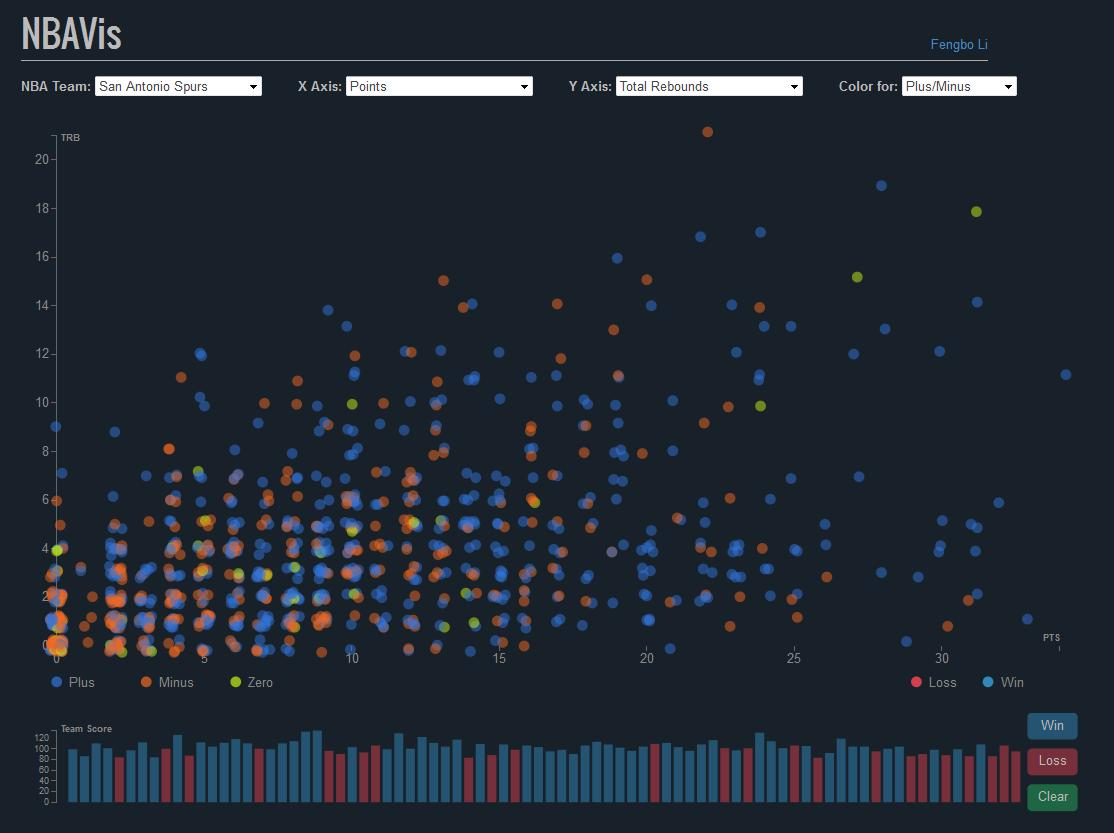
\includegraphics[width=\linewidth]{georgiatech.jpg}
\end{figure}


\subsection{In Entertainment}



\section{Method/Computational Model}
\subsection{Method Overview}
\emph{Figure 2} is a flow chart diagram of the components necessary to program an interface with three graphs. The first graph is a radar chart that corresponds to a player's assists per game (APG), steals per game (SPG), blocks per game (BPG), rebounds per game (RPG), and turnovers per game (TPG). The second graph is a bar chart that corresponds to a player's average points per game (PPG) versus the average player's average points per game. This bar chart is presented vertically. The third graph is the same as the second bar chart, except rather than presented vertically, it is presented horizontally. For each node in the flow chart diagram, there is a subsection within this section that corresponds to an explanation of how this step in the software engineering process was approached. 

\begin{figure}[h]
\caption{A flow chart diagram of our programming process.}
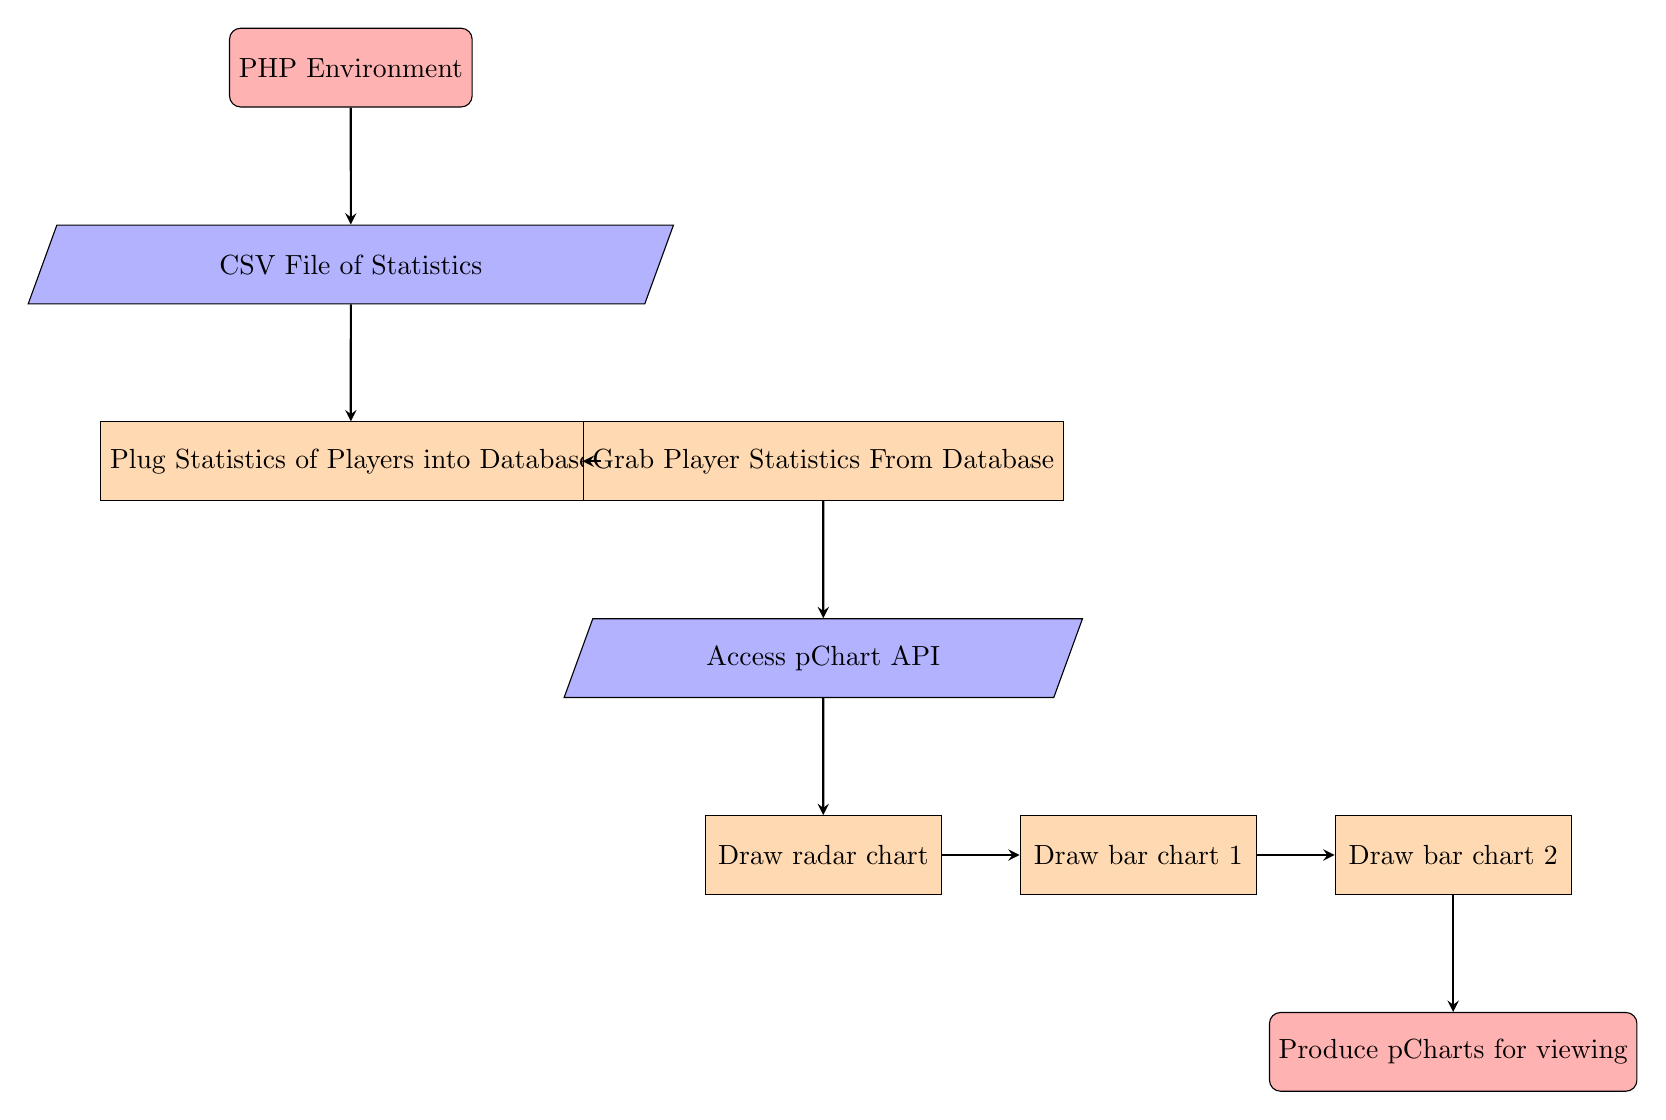
\begin{tikzpicture}[node distance=2cm]

\node (start) [startstop] {PHP Environment};
\node (in1) [io, below of=start, yshift=-0.5cm] {CSV File of Statistics};
\node (pro1) [process, below of=in1, yshift=-0.5cm] {Plug Statistics of Players into Database};
\node (pro2) [process, right of=pro1, xshift=4cm] {Grab Player Statistics From Database};
\node (in2) [io, below of=pro2, yshift=-0.5cm] {Access pChart API};
\node (pro3) [process, below of=in2, yshift=-0.5cm] {Draw radar chart};
\node (pro4) [process, right of=pro3, xshift=2cm] {Draw bar chart 1};
\node (pro5) [process, right of=pro4, xshift=2cm] {Draw bar chart 2};
\node (stop) [startstop, below of=pro5, yshift=-0.5cm] {Produce pCharts for viewing};

\draw [arrow] (start) -- (in1);
\draw [arrow] (in1) -- (pro1);
\draw [arrow] (pro1) -- (pro2);
\draw [arrow] (pro2) -- (in2);
\draw [arrow] (in2) -- (pro3);
\draw [arrow] (pro3) -- (pro4);
\draw [arrow] (pro4) -- (pro5);
\draw [arrow] (pro5) -- (stop);
\end{tikzpicture}
\end{figure}



\subsection{PHP Environment}
This node is the start block that represents how each subsequent step can be completed. In order to satisfy the following requirements, we must operate in a PHP environment.
\subsection{CSV File of Statistics}
An input block, this node represents the NBA statistics we require to generate meaningful charts. In our file "Document2.csv", we have entries consisting of players like James Harden, Danilo Gallinari, and Jordan Clarkson with statistics ranging from their PPG to their RPG.
\subsection{Plug Statistics of Players into Database}
In order to do anything meaningful with the data we gathered in our CSV, we must place the data into a database for later use in the pChart environment. To do this, we have a file "insert\_nba.php" that uses mySQL to connect to a database, parse our .csv file, and place it into a table called player\_info. Some code pertaining to these steps:
To connect to the database:
\begin{lstlisting}
$user = 'root';
$pass ='' ; 
$db = 'nba';
mysql_connect('localhost',$user,$pass);
mysql_select_db($db);
\end{lstlisting}
To parse our .csv file:
\begin{lstlisting}
$parsed_data = array_map('str_getcsv',
file('Document2.csv'));
\end{lstlisting}
Finally, to place the data into a table:
\begin{lstlisting}
$ins_sql = "INSERT INTO player_info (name,age
,team_name,wins,loss,ppg,bpg,rpg,apg,tpg,spg,
games) VALUES ('$name','$age','$team','$wins'
,'$loss','$ppg','$bpg','$rpg','$apg','$tpg',
'$spg','$games')";
\end{lstlisting}

\subsection{Grab Player Statistics From Database}
Naturally, it is necessary to access the database we have created in order to use our data for chart generation. This step happens at a similar time as the next step, so there is not necessarily a temporal order. As a code example of this step, let's look at a method in our file "vis\_proj.php" file that averages the points per game of a player:
\begin{lstlisting}
 function get_average_ppg(){
 	$avg_sql = "SELECT ppg 
	FROM player_info";
 	
	$result = mysql_query($avg_sql);
 	$result = mysql_fetch_assoc($result);
 	$sum = 0;
 	foreach($result as $key => $value){
 		$sum += $value;
 	}
 	$avg = $sum/count($result);
  	return $avg;
 }
\end{lstlisting}

\subsection{Access pChart API}
In order to generate the charts that we want, we utilized pChart. Accessing this API consisted of the following include statements in our "vis\_proj" file:
\begin{lstlisting}
include("pChart2.1.4/pChart2.1.4/class/pData
.class.php");
include("pChart2.1.4/pChart2.1.4/class/pDraw
.class.php");
include("pChart2.1.4/pChart2.1.4/class/pRadar
.class.php");
include("pChart2.1.4/pChart2.1.4/class/pImage
.class.php");
\end{lstlisting}
\subsection{Draw radar chart, bar chart 1, bar chart 2}
To draw our charts, we utilized pChart's functionalities. Let us explain the proess of drawing the radar chart. First, we initialized a pRadar object. Then, we passed this object into a function along with a player's data. In this function, we used the pChart method "setGraphArea" to specify the size of the graph, created an Options object to hold specifications for what we wanted our graph to look like, and then finally passed our pRadar object into the "drawRadar" pChart function.
\subsection{Produce pCharts for viewing}
This node is the completion of the process of generating charts, a result of compiling the programs outlined in the previous steps. Three charts corresponding to a player are presented to the user.
\subsection{Parameters}
Since our visualization module uses static data that we gathered via a basketball statistics website, our parameters to pChart functions are unchanging. 
\section{Implementation}
In implementing our visualization software, we were surprised to see how many different options for packages there were. Initially, we planned on using Python embedded in HTML in order to use the pyfigure package, but we eventually landed on using pCharts due to its ability to be implemented in a PHP context. We also wanted to include salary in our radar chart but found it virtually impossible to find a reasonable way to describe statistics and salary using the same units due to their large difference in size. 
\section{Results and Performance}
\subsection{Results}
\begin{figure}[h]
\caption{A visualization of James Harden's performance in the NBA.}
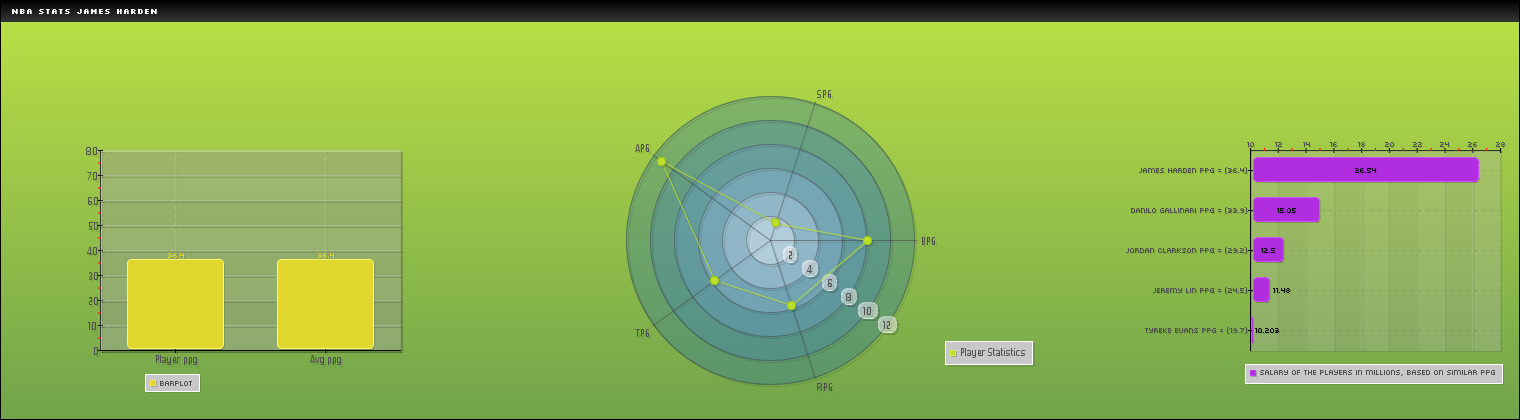
\includegraphics[width=\linewidth]{JamesHarden.png}
\end{figure}
We can see in \emph{Figure 1} an example of what our module produces. In the left chart, we can see that James Harden averages many more points than the average player. In our radar chart, we easily get, through our visual sense, an idea of what kind of player James Harden is: he averages many assists, he doesn't get many steals or rebounds, and he turns the ball over seldolmy. Finally, on the right, we see a bar chart of a sample comparison we can make between 
\subsection{Performance Analysis}
Since our module does not make use of I/O dependent on the user, and because our data set is reasonably small, a performance analysis of the generation of charts is not necessary.
\section{Conclusions and Future Work}
From our survey of the current visualization research landscape, we see that no other publications have used graphs like radar charts in order to analyze the performance of an NBA player as well as the worth of the player, as judged by salary. In fact, our survey shows us that using visualization techniques to effectively describe NBA players is oddly underdeveloped in the visualization research community. As such, we hope that the novelty of our module inspires others to make NBA visualizations a more robust field. The value of such visualizations are that NBA executives can cite these graphs of players in order to make reasoned judgments on how much they should spend on a specific player. Naturally, since each team must operate within a salary cap, the ability to use visualizations such as these in order to make financially sound decisions is a major advantage to any team that chooses to embrace it.
\subsection{Future Work}
Since this is a novel work in the realm of visualization research, future opportunities to expand the field of NBA visualization using this as a platform to build off of are plentiful. Visualizations that look into more advanced statistics could allow more concrete conclusions about a player's worth. Additionally, a module that allows for a user to select any player in the NBA and generates these graphs for him would be a big step forward. A wider variety of graphs and charts dedicated to each player would also be helpful in drawing conclusions.
\newpage
\bibliographystyle{abbrv-doi}
\bibliography{template}


\begin{figure}[h]
\caption{A flow chart diagram of our programming process.}
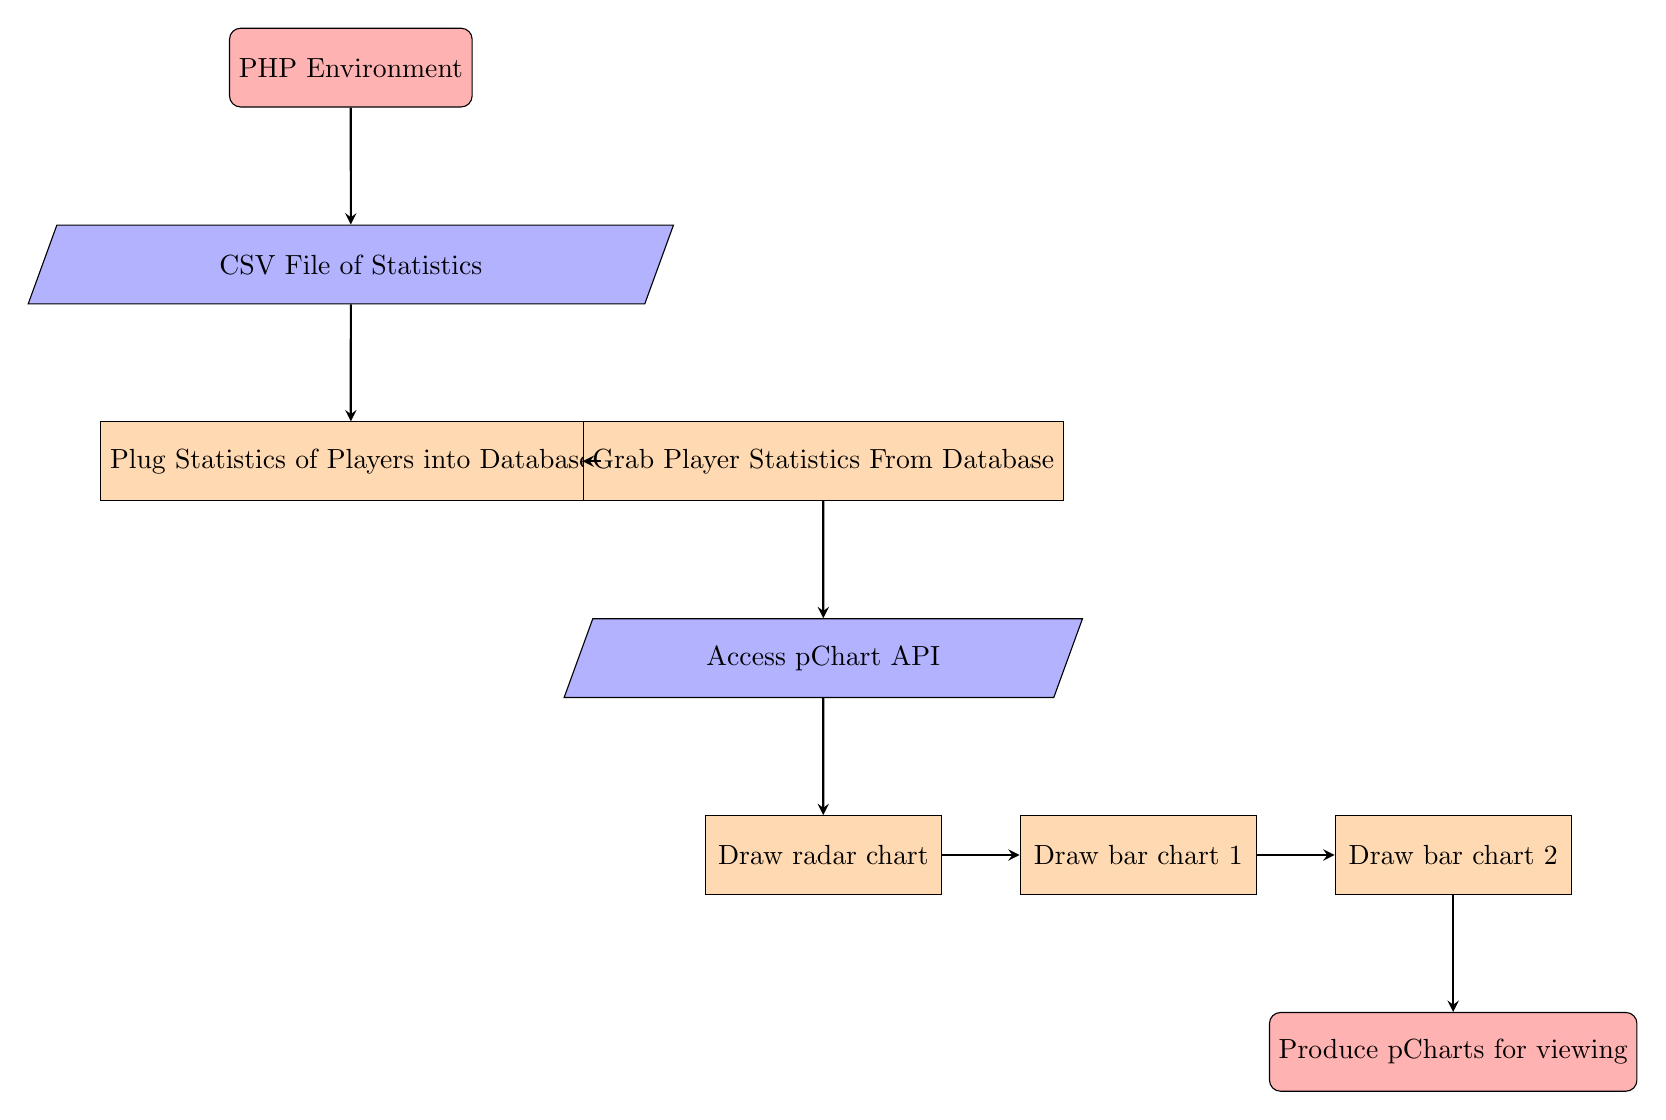
\begin{tikzpicture}[node distance=2cm]

\node (start) [startstop] {PHP Environment};
\node (in1) [io, below of=start, yshift=-0.5cm] {CSV File of Statistics};
\node (pro1) [process, below of=in1, yshift=-0.5cm] {Plug Statistics of Players into Database};
\node (pro2) [process, right of=pro1, xshift=4cm] {Grab Player Statistics From Database};
\node (in2) [io, below of=pro2, yshift=-0.5cm] {Access pChart API};
\node (pro3) [process, below of=in2, yshift=-0.5cm] {Draw radar chart};
\node (pro4) [process, right of=pro3, xshift=2cm] {Draw bar chart 1};
\node (pro5) [process, right of=pro4, xshift=2cm] {Draw bar chart 2};
\node (stop) [startstop, below of=pro5, yshift=-0.5cm] {Produce pCharts for viewing};

\draw [arrow] (start) -- (in1);
\draw [arrow] (in1) -- (pro1);
\draw [arrow] (pro1) -- (pro2);
\draw [arrow] (pro2) -- (in2);
\draw [arrow] (in2) -- (pro3);
\draw [arrow] (pro3) -- (pro4);
\draw [arrow] (pro4) -- (pro5);
\draw [arrow] (pro5) -- (stop);
\end{tikzpicture}
\end{figure}


\end{document}

